\chapter{Ring Theory}
\setcounter{equation}{0}
\setcounter{table}{0}
\setcounter{figure}{0}

\section{Brief Discussion on Bezout Domain, PID, UFD, gcd, lcm}
The concept of gcd and lcm can be generalized to UFDs. We use the definition $ gcd(a,b)=d $ iff $ d $ divides $ a,b $ and $ x\mid a$, $x\mid b \implies x\mid d $. Similarly, $ a,b $ divides the lcm and  $ a\mid x $, $ b\mid x $ implies $ lcm(a,b)\mid x $. We can show that $ ab= gcd(a,b)lcm(a,b) $. 
\begin{theorem}
	$ ab= gcd(a,b)lcm(a,b) $ in UFD.
\end{theorem}
\begin{proof}
	Let $ gcd(a,b)=d $. $ a=da',b=db' $. We have some results from the definition of gcd.\\
	$ gcd(a',b')=1 $ since $ u\mid a',b' \implies a'=ux_1, b'=ux_2 \implies a= dux_1, b= dux_2 \implies du\mid a,b\implies du\mid d \implies u$ is unit.\\
	So, enough to prove $ lcm(a,b) = da'b' $. Since both $ a,b $ divides $ da'b' $ and $ a,b \mid x \implies x=da'k_1=db'k_2$ By uniqueness of factors $ a'k_1= b'k_2 $. $ gcd(a',b')=1 \implies b'\mid k_1 $ by irreducible factor decomposition argument. So, $ x=da'b'k $ i.e. $ da'b' $ divides $ x $. So, $ ab=d^2a'b'= gcd\cdot lcm $ 
\end{proof}
\begin{definition}
	A integral domain is called Bezout domain if sum of any two principal ideals is principal. i.e. $ (a,b)=(d) $ for any $ a,b\in R $. The Bezout's identity holds for this case: $ d= ua+vb $ for some $ u,v\in R $. In general any finitely generated ideal is principal.
\end{definition}

A Bezout domain need not be Noetherian or UFD. For example ring of Algebraic integers is not UFD(any element is not irreducible since it's square root is also algebraic integer). Any PID is by definition Bezout domain. If $ R $ is a Bezout domain then TFAE:
\begin{itemize}
	\item $ R $ is PID
	\item $ R $ is Noetherian 
	\item $ R $ is UFD
\end{itemize}

So, a Bezout UFD is a PID. Example of non-Bezout UFD is $ \Z[x] $. Consider $ (2,x) $.

Now we will discuss a little bit about properties that hold in a PID(not necessarily in UFD):
\begin{theorem}
	$ R $ is a PID. $ (a)+(b)=(a,b)= (gcd(a,b)) $ and $ (a)\cap(b)= (lcm(a,b)) $. 
\end{theorem}
\begin{proof}
	One side inclusion is true for general UFDs.\\
	Since $ gcd(a,b)\mid a,b $, $ a,b\in (gcd(a,b)) \implies (a,b)\subseteq (gcd(a,b)) $.\\
	On the other hand, let $ (a,b)=(d) $ by definition of PID. $ a,b\in (d) \implies d\mid a$ ,  $d\mid b $. So, by definition of gcd, $ d\mid gcd(a,b) \implies (gcd(a,b))\subseteq (d)$. This side is not true for UFD in general. Take $ gcd(2,x)=1 $ in $ \Z[x] $.\\
	This also gives rise to the famous Bezout's identity $ gcd(a,b)= ax+by $ for some $ x,y\in R $.\\
	$ a,b\mid lcm(a,b) \implies lcm(a,b)\subseteq (a), (b)$. And $ (a)\cap(b)=(m)\implies a,b\mid m  \implies lcm(a,b)\mid m \implies (m) \subseteq (lcm(a,b))$. The second step uses the property of PID.
\end{proof}
\newpage
\section{Solution}
\textbf{R1:} Let $R=\mathbb{Z}[\sqrt{-3}]=\{a+b \sqrt{-3}: a, b \in \mathbb{Z}\}$.\\
(a) Why is $R$ an integral domain?\\
(b) What are the units in $R$ ?\\
(c) Is the element 2 irreducible in $R$ ?\\
(d) If $x, y \in R$, and 2 divides $x y$, does it follow that 2 divides either $x$ or $y$ ? Justify your answer.
\soln Let $ R=\Z[\sqrt{-3}] $
\begin{itemize}
	\item[(a)] Let $ (a+b\sqrt{-3})(c+d\sqrt{-3})=0\implies ac-3bd +\sqrt{-3}(ad+bc) = 0\implies \dfrac{a}{d}=\dfrac{3b}{c}=3k $\\
	This implies $ 3kd^2 + kc^2=0 \implies k=0$ or $ c=d=0 $. $ k=0\implies a=b=0 $, So, one of the factor is $ 0 $. 
	\item[(b)] Let $ (a+b\sqrt{-3})(c+d\sqrt{-3})=1 \implies (a-b\sqrt{-3})(c-d\sqrt{-3})=1 \implies (a^2 +3b^2)(c^2+3d^2)=1\implies b=d=0, a=c=\pm 1 $. So, the only units are $ \pm 1 $.
	\item[(c)] $ \alpha\beta=2 \implies \bar{\alpha}\bar{\beta}=2 \implies 4= \mid\alpha\mid^2\mid\beta\mid^2$. This gives us that one of them is a unit.
	\item[(d)] $ (1+\sqrt{-3})(1-\sqrt{-3})=4 $. But $ 2 $ doesn't divide the elements individually.
\end{itemize}
\qed\\
\textbf{R2:} 
\begin{itemize}
	\item[(a)] Give an example of an integral domain with exactly 9 elements.
	\item[(b)] Is there an integral domain with exactly 10 elements? Justify your answer. 
\end{itemize}
\soln
Finite integral domains are fields. Finite fields are of prime powers.
\begin{itemize}
	\item[(a)] $ \mathbb{F}_9=\mathbb{F}_3[x]/(x^2+1) $.
	\item[(b)] Not possible.
\end{itemize} 
\qed\\
\textbf{R3.1:} Let

$$
F=\left\{\left[\begin{array}{cc}
	a & b \\
	2 b & a
\end{array}\right]: a, b \in \mathbb{Q}\right\} .
$$

\begin{itemize}
	\item[(a)] Prove that $F$ is a field under the usual matrix operations of addition and multiplication.
	\item[(b)] Prove that $F$ is isomorphic to the field $\mathbb{Q}(\sqrt{2})$.
\end{itemize}
\textbf{R3.2:} Let $\mathbb{F}$ be a field and let $R=\mathbb{F}[X, Y]$ be the ring of polynomials in $X$ and $Y$ with coefficients from $\mathbb{F}$.
\begin{itemize}
	\item[(a)] Show that $M=\langle X+1, Y-2\rangle$ is a maximal ideal of $R$.
	\item[(b)] Show that $P=\langle X+Y+1\rangle$ is a prime ideal of $R$.
	\item[(c)] Is $P$ a maximal ideal of $R$ ? Justify your answer.
\end{itemize}

\soln
We only need to verify multiplication and inverse.
\begin{itemize}
	\item[1.a] $$ \matr{a_1}{b_1}{2b_1}{a_1}\matr{a_2}{b_2}{2b_2}{a_2}=\matr{a_1a_2 + 2b_1b_2}{a_1b_2+b_1a_2}{2a_1b_2+2b_1a_2}{2b_1b_2+a_1a_2}\in F $$. \\
	Let $ \matr{a}{b}{2b}{a}\ne \matr{0}{0}{0}{0}\implies a^2 -2b^2 \ne 0 $.
	$$ \matr{a}{b}{2b}{a}^{-1}= \frac{1}{a^2-2b^2}\matr{a}{-b}{-2b}{a}\in F $$
	\item[1.b] $$ \matr{a}{b}{2b}{a}\mapsto a + b\sqrt{2} $$ Check the multiplication.
	\item[2.a] Let $ \varphi: R \to \mathbb{F} $ given by $ \varphi(x) = -1, \varphi(y)=2 $. We show that kernel is $ M $ and image is full(clearly), FIT implies that $ R/M \cong \mathbb{F} \implies M $ is maximal.\\
	$ <x+1,y-2>\subseteq ker(\varphi) $. Let $ \varphi(f(x,y))=0 $. $ f(x,y)= h(y)+ (x-1)g(x,y) $.\\
	$ f(-1,2)=0 \implies h(2)=0 \implies (y-2)\mid h(y)$. This proves that the kernel is $ <x+1,y-2> $.\\
	\textbf{Alternatively:} $$ \dfrac{\mathbb{F}[x,y]}{(x+1,y-2)} \cong \dfrac{\mathbb{F}[x][y]/(y-2)}{(x+1,y-2)/(y-2)} \cong \dfrac{\mathbb{F}[x]}{(x-1)} \cong \mathbb{F} $$
	\item[2.b] $ R/P \cong \mathbb{F}[x] $ integral domain implies $ P $ is prime.\\
	($ \phi: R \to \mathbb{F}[x] $ with $ x\mapsto x, y \mapsto -(x+1) $. $ \phi(f(x,y))=0 \implies F(y)$ as a polynomial of $ y $ has a root at $ (-x-1) \implies (y+x+1) \mid f $, this shows the kernel is equal to $ P $).
	\item[2.c] From the previous solution we can already see $ R/P $ is not a field. Alternatively, $ P\subsetneq (x+1,y) $.  
\end{itemize}
\qed\\
\textbf{R4:} Let $R$ be an integral domain containing a field $k$ as a subring. Suppose that $R$ is a finite-dimensional vector space over $k$, with scalar multiplication being the multiplication in $R$. Prove that $R$ is a field.\\
\soln Let the dimension of $ R $ over $ k $ be $ n $. Let $ r\in R $ be a nonzero vector. $ 1,r,\cdots,r^{n} $ are linearly dependent. $$ a_0 + \cdots + a_n r^n = 0$$ with some $ a_i $ nonzero. We see that $ a_0=0 \implies r(\cdots)=0 \implies a_i =0$ for all $ i $. \\
So, $ a_0 \ne 0 \implies 1 = r(a_0^{-1})(\cdots) \implies r$ is a unit.\\
\textbf{Alternative Proof:} Let $ \phi: R\to R $ be given by multiplication by $ r $. Easy to show that it is a $ k $-linear map of vector spaces, i.e. $ ker(\phi)=0 $ implies injective implies surjective(rank nullity theorem) for finite dimensional case. This implies there is a preimage of $ 1 $. So, $ rx=1 $ for some $ x\in R $.   
\qed\\
\newpage
\textbf{R5:} Let $R$ be a commutative ring with identity and let $I$ and $J$ be ideals of $R$.\\
\begin{itemize}
	\item[(a)] Define
$$
(I: J)=\{r \in R: r x \in I \text { for all } x \in J\}
$$
Show that $(I: J)$ is an ideal of $R$ containing $I$.
	\item[(b)] Show that if $P$ is a prime ideal of $R$ and $x \notin P$, then $(P:\langle x\rangle)=P$, where $\langle x\rangle$ denotes the principal ideal generated by $x$.
	\item[(c)] Define what is meant by the sum $I+J$ and the product $I J$ of the ideals $I$ and $J$.
	\item[(d)] If $I$ and $J$ are distinct maximal ideals, show that $I+J=R$ and $I \cap J=I J$.
\end{itemize}

\soln

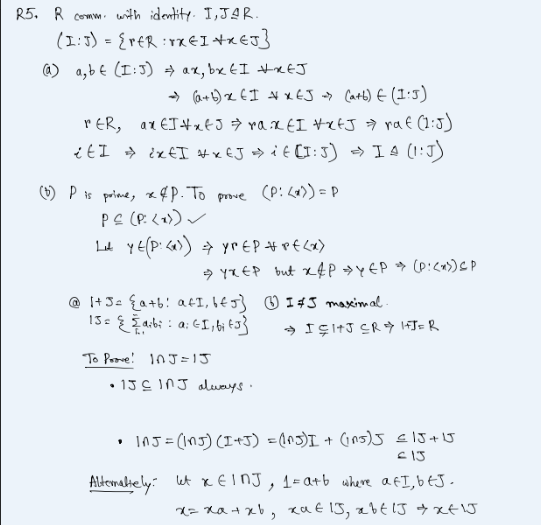
\includegraphics{R2.5.png}
\qed\\
\textbf{R6:} Let $\mathbb{F}_{2}$ be the field with 2 elements.
\begin{itemize}
	\item[(a)] Show that $f(X)=X^{3}+X^{2}+1$ and $g(X)=X^{3}+X+1$ are the only irreducible polynomials of degree 3 in $\mathbb{F}_{2}[X]$.
	\item[(b)] Give an explicit field isomorphism

$$
\mathbb{F}_{2}[X] /\langle f(X)\rangle \cong \mathbb{F}_{2}[X] /\langle g(X)\rangle
$$
\end{itemize}
\soln
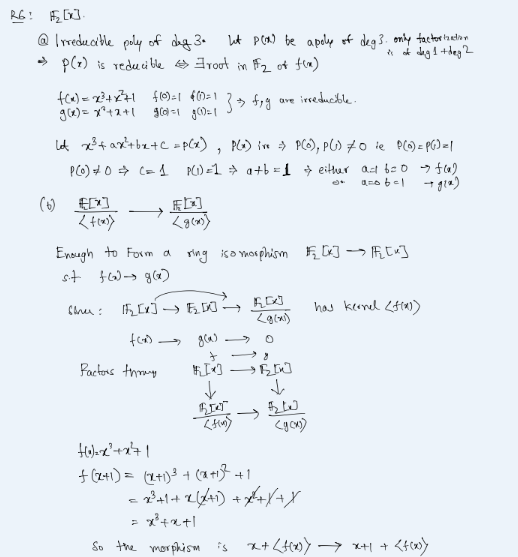
\includegraphics{R2.6.png}
\qed\\ 
\textbf{Find the solution for the rest of the problems on: }
%R7. Show that $\mathbb{Z}[i] /\langle 1+i\rangle$ is isomorphic to the field $\mathbb{F}_{2}$ with 2 elements. As usual, $i$ denotes the complex number $\sqrt{-1}$ and $\langle 1+i\rangle$ denotes the principal ideal of $\mathbb{Z}[i]$ generated by $1+i$.\\
%R8. Consider the ring $\mathbb{Z}[X]$ of polynomials in one variable $X$ with coefficients in $\mathbb{Z}$.\\
%(a) Find all the units of $\mathbb{Z}[X]$.\\
%(b) Describe an easy way to recognize the elements of the ideal $I$ of $\mathbb{Z}[X]$ generated by 2 and $X$.\\
%(c) Find a prime ideal of $\mathbb{Z}[X]$ that is not maximal.
%
%R9. Determine, with justification, all of the irreducible polynomials of degree 4 over the field $\mathbb{F}_{2}$ of two elements.\\
%R10. Let $R=\mathbb{Z}[\sqrt{-10}]$.\\
%(a) Show that $R$ is not a PID. (Hint: Show that 10 admits two essentially different factorizations into irreducible elements of $R$.)\\
%(b) Let $P=\langle 7,5+\sqrt{-10}\rangle$. Show that $R / P$ is isomorphic to $\mathbb{Z} / 7 \mathbb{Z}$.
%
%R11. Suppose that $R$ is an integral domain and $X$ is an indeterminate.\\
%(a) Prove that if $R$ is a field, then the polynomial ring $R[X]$ is a PID (principal ideal domain).\\
%(b) Show, conversely, that if $R[X]$ is a PID, then $R$ is a field.
%
%R12. (a) Prove that every Euclidean domain is a principal ideal domain (PID).\\
%(b) Give an example of a unique factorization domain that is not a PID and justify your answer.
%\soln
%\qed\\
%\textbf{R13:}
%\begin{itemize}
%	\item[(a)] Show that for each natural number $n \in \mathbb{N}$, there is an irreducible polynomial $P_{n}(X) \in \mathbb{Q}[X]$ of degree $n$.\\
%	\item[(b)] Is this true when $\mathbb{Q}$ is replaced by $\mathbb{R}$ ? Explain. 
%\end{itemize} 
%\soln Remember the Eisenstein Criterion and Gauss Lemma. Let $ p(x)=a_nx^n +\cdots +a_0 $ be such that a prime $ p $ divides $ a_0,\cdots, a_{n-1}, p\nmid a_n, p^2\nmid a_0 $ then the polynomial is irreducible over $ \Z $ or $ \Q $.
%\begin{itemize}
%	\item[(a)] Let $ P_n(X)= X^n + 2 $
%	\item[(b)] This is not true for $ \R $. The maximum degree of irreducible polynomial over $ \R $ is $ 2 $. E.g. $ x^2+1 $.
%\end{itemize}
%\qed\\
%\textbf{R14:} Let $R$ be a commutative ring with identity. If $I \subseteq R$ is an ideal, then the radical of $I$, denoted $\sqrt{I}$, is defined by
%
%$$
%\sqrt{I}=\left\{a \in R: a^{n} \in I \text { for some positive integer } n\right\}
%$$
%
%(a) Prove that $\sqrt{I \cap J}=\sqrt{I} \cap \sqrt{J}$.\\
%(b) If $P$ is a prime ideal of $R$ and $r \in \mathbb{N}$, find $\sqrt{P^{r}}$ and justify your answer.\\
%(c) Find $\sqrt{I}$, where $I$ is the ideal $\langle 108\rangle$ in the ring $\mathbb{Z}$ of integers.
%
%R15. (a) Show that $\mathbb{Z}[i] /\langle 3+i\rangle \cong \mathbb{Z} / 10 \mathbb{Z}$, where $i$ is the usual complex number $\sqrt{-1}$.\\
%(b) Is $\langle 3+i\rangle$ a maximal ideal of $\mathbb{Z}[i]$ ? Give a reason for your answer.
%
%R16. Let $R=\mathbb{Z}[X]$. Answer the following questions about the ring $R$. You may quote an appropriate theorem, provide a counterexample, or give a short proof to justify your answer.\\
%(a) Is $R$ a unique factorization domain?\\
%(b) Is $R$ a principal ideal domain?\\
%(c) Find the group of units of $R$.\\
%(d) Find a prime ideal of $R$ which is not maximal.\\
%(e) Find a maximal ideal of $R$.
%
%R17. An element $a$ in a ring $R$ is nilpotent if $a^{n}=0$ for some natural number $n$.\\
%(a) If $R$ is a commutative ring with identity, show that the set of nilpotent elements forms an ideal.\\
%(b) Describe all of the nilpotent elements in the ring $\mathbb{C}[X] /\langle f(X)\rangle$, where
%
%$$
%f(X)=(X-1)\left(X^{2}-1\right)\left(X^{3}-1\right)
%$$
%
%(c) Show that part (a) need not be true if $R$ is not commutative. (Hint: Try a matrix ring.)
%
%R18. Let $R$ be a ring, let $R^{*}$ be the set of units of $R$, and let $M=R \backslash R^{*}$. If $M$ is an ideal, prove that $M$ is a maximal ideal and that moreover it is the only maximal ideal of $R$.\\
%R19. (a) Let $R$ be a PID and let $I, J$ be nonzero ideals of $R$. Show that $I J=I \cap J$ if and only if $I+J=R$.\\
%(b) Show that $\mathbb{Z} / 900 \mathbb{Z}$ is isomorphic to $\mathbb{Z} / 100 \mathbb{Z} \oplus \mathbb{Z} / 9 \mathbb{Z}$ as rings.\\
%(a) Let $I=\left\langle X^{2}+2,5\right\rangle \subseteq \mathbb{Z}[X]$ and let $J=\left\langle X^{2}+2,3\right\rangle$. Show that $I$ is a maximal ideal, but $J$ is not a maximal ideal.\\
%R20. Let $F$ be a subfield of a field $K$ and let $f(X), g(X) \in F[X] \backslash\{0\}$. Prove that the greatest common divisor of $f(X)$ and $g(X)$ in $F[X]$ is the same as the greatest common divisor taken in $K[X]$.\\
%R21. Find the greatest common divisor of $X^{3}-6 X^{2}+X+4$ and $X^{5}-6 X+1$ in $\mathbb{Q}[X]$.\\
%R22. Define $\varphi: \mathbb{C}[X, Y] \rightarrow \mathbb{C}[T]$ by $\varphi(X)=T^{2}, \varphi(Y)=T^{3}$.\\
%(a) Show that $\operatorname{Ker}(\varphi)=\left\langle Y^{2}-X^{3}\right\rangle$.\\
%(b) Find the image of $\varphi$.
%
%R23. Prove that $\mathbb{Z}[\sqrt{-2}]$ is a Euclidean domain.\\
%R24. Let $m, n$ be two non-zero integers. Prove that the greatest common divisor of $m$ and $n$ in $\mathbb{Z}$ is the same as the greatest common divisor taken in $\mathbb{Z}[i]$. Generalize this to a statement about the greatest common divisor of elements $a$ and $b$ in a Euclidean domain $R$ which is a subring of a Euclidean domain $S$.
%
%R25. Prove that the center of the matrix ring $M_{n}(\mathbb{R})$ is the set of scalar matrices, i.e., $C\left(M_{n}(\mathbb{R})\right)=\left\{a I_{n}\right.$ : $a \in \mathbb{R}\}$.
%
%R26. Let $R_{1}=\mathbb{F}_{p}[X] /\left\langle X^{2}-2\right\rangle$ and $R_{2}=\mathbb{F}_{p}[X] /\left\langle X^{2}-3\right\rangle$ where $\mathbb{F}_{p}$ is the field of $p$ elements, $p$ a prime. Determine if $R_{1}$ is isomorphic to $R_{2}$ in each of the cases $p=2, p=5$, and $p=11$.\\
%R27. (a) Show that the only automorphism of the field $\mathbb{R}$ of real numbers is the identity.\\
%(b) Show that any automorphism of the field $\mathbb{C}$ of complex numbers which fixes $\mathbb{R}$ is either the identity or complex conjugation.\\
%R28. (a) Find all ideals of the ring $\mathbb{Z} / 24 \mathbb{Z}$.\\
%(b) Find all ideals of the ring $\mathbb{Q}[X] /\left\langle X^{2}+2 X-2\right\rangle$.
%
%R29. Let $R$ be an integral domain. Show that the group of units of the polynomial ring $R[X]$ is equal to the group of units of the ground ring $R$.\\
%R30. Express the polynomial $X^{4}-2 X^{2}-3$ as a product of irreducible polynomials over each of the following fields: $\mathbb{Q}, \mathbb{R}, \mathbb{C}, \mathbb{F}_{5}$.\\
%R31. Let $\omega=(1+\sqrt{-3}) / 2 \in \mathbb{C}$ and let $R=\{a+b \omega: a, b \in \mathbb{Z}\}$.\\
%(a) Show that $R$ is a subring of $\mathbb{C}$.\\
%(b) Show that $R$ is a Euclidean domain with respect to the norm function $N(z)=z \bar{z}$, where, as usual, $\bar{z}$ denotes the complex conjugate of $z$.\\
%R32. Let $I$ be an ideal of $\mathbb{R}[X]$ generated by an irreducible polynomial of degree 2 . Show that $\mathbb{R}[X] / I$ is isomorphic to the field $\mathbb{C}$.\\
%R33. Show that in the ring $M$ of $2 \times 2$ real matrices (with the usual sum and multiplication of matrices), the only 2 -sided ideals are $\langle 0\rangle$ and the whole ring $M$.\\
%R34. Let $R$ be a commutative ring with identity. Suppose $a \in R$ is a unit and $b \in R$ is nilpotent. Show that $a+b$ is a unit.\\
%R35. (b) Let $R$ and $S$ be commutative rings with identities $1_{R}$ and $1_{S}$, respectively, let $f: R \rightarrow S$ be a ring homomorphism such that $f\left(1_{R}\right)=1_{S}$. If $P$ is a prime ideal of $S$ show that $f^{-1}(P)$ is a prime ideal of $R$.\\
%(c) Let $f$ be as in part (b). If $M$ is a maximal ideal of $S$, is $f^{-1}(M)$ a maximal ideal of $R$ ? Prove that it is or give a counterexample.\\
%R36. (a) Let $\mathbb{H}$ be the ring of quaternions, $q=a+b \mathbf{i}+c \mathbf{j}+d \mathbf{k}$, where $\mathbf{i}^{2}=\mathbf{j}^{2}=\mathbf{k}^{2}=\mathbf{i j k}=-1,, a, b, c, d \in \mathbb{R}$. Let $q^{*}=a-b \mathbf{i}-c \mathbf{j}-d \mathbf{k}$ and $\|q\|^{2}=q q^{*}=a^{2}+b^{2}+c^{2}+d^{2}$. Show that the set $\mathbb{H}_{1}$ of quaternions with $\|q\|=1$ is a group under quaternion multiplication. Hint: show $\left(q_{1} q_{2}\right)^{*}=q_{2}^{*} q_{1}^{*}$ and use $q^{* *}=q, a^{*}=a$ for $a \in \mathbb{R}$.\\
%(b) Show that the map
%
%$$
%\mathbb{H} \rightarrow M_{2}(\mathbb{C}), \quad q=a+b \mathbf{i}+c \mathbf{j}+d \mathbf{k} \mapsto M(q):=\left[\begin{array}{cc}
%	a+b i & c+d i \\
%	-c+d i & a-b i
%\end{array}\right] \quad i=\sqrt{-1},
%$$
%
%is an $\mathbb{R}$-algebra homomorphism, and that $\|q\|^{2}=\operatorname{det} M(q)$.\\
%R37. Let $\mathbb{H} \rightarrow M_{2}(\mathbb{C})$ be the ring homomorphism of part (b) of problem R40. Show that this induces an isomorphism
%
%$$
%\mathbb{H}_{1} \cong S U_{2}=\left\{T \in M_{2}(\mathbb{C}) \mid T^{t} \bar{T}=I_{2}, \operatorname{det} T=1\right\}
%$$
%
%R38. Let $\mathbb{H}_{1} \rightarrow S U_{2}$ be the isomorphism of R 41 . For each $q \in \mathbb{H}_{1}$, define a map $\mathbb{R}^{3} \rightarrow \mathbb{R}^{3}$ :
%
%$$
%\mathbf{v}=\left(\begin{array}{l}
%	a \\
%	b \\
%	c
%\end{array}\right) \mapsto R_{q}(\mathbf{v})=\left(\begin{array}{l}
%	a^{\prime} \\
%	b^{\prime} \\
%	c^{\prime}
%\end{array}\right)
%$$
%
%by the rule $q(a \mathbf{i}+b \mathbf{j}+c \mathbf{k}) q^{*}=a^{\prime} \mathbf{i}+b^{\prime} \mathbf{j}+c^{\prime} \mathbf{k}$. Show that this makes sense: the quaternion $q(a \mathbf{i}+b \mathbf{j}+c \mathbf{k}) q^{*}$ has only $\mathbf{i}, \mathbf{j}, \mathbf{k}$ components. The $\operatorname{map} \mathbf{v} \mapsto R_{q}(\mathbf{v})$ is clearly an invertible $\mathbb{R}$-linear map, hence an element of $G L(3, \mathbb{R})$. Now show that it preserves the dot-product of vectors in $\mathbb{R}^{3},\left(a_{1}, b_{1}, c_{1}\right) \cdot\left(a_{2}, b_{2}, c_{2}\right)=$ $a_{1} a_{2}+b_{1} b_{2}+c_{1} c_{2}$, that is
%
%$$
%R_{q}\left(\mathbf{v}_{1}\right) \cdot R_{q}\left(\mathbf{v}_{2}\right)=\mathbf{v}_{1} \cdot \mathbf{v}_{2} .
%$$
%
%Hint: Let quat $(a, b, c)=a \mathbf{i}+b \mathbf{j}+c \mathbf{k}$, then
%
%$$
%\mathbf{v}_{1} \cdot \mathbf{v}_{2}=\left[\operatorname{quat}\left(\mathbf{v}_{1}\right) \operatorname{quat}\left(\mathbf{v}_{2}\right)^{*}+\operatorname{quat}\left(\mathbf{v}_{2}\right) \operatorname{quat}\left(\mathbf{v}_{1}\right)^{*}\right] / 2 .
%$$
%
%Therefore $R_{q} \in S O_{3}(\mathbb{R})=\left\{T \in M_{3}(\mathbb{R}) \mid T^{t} T=I_{3}, \operatorname{det} T=1\right\}$.\\
%R39. Show that the map $q \mapsto R_{q}$ is a homomorphism $\mathbb{H}_{1} \rightarrow S O(3, \mathbb{R})$, i.e., $R_{q_{1} q_{2}}=R_{q_{1}} R_{q_{2}}$. Show that it induces an isomorphism $S U_{2} / \pm 1 \cong S O(3, \mathbb{R})$.